% author: Tomas Trnka
% mail: tomas@trnkatomas.eu
% date: 2013-07-04

\documentclass[a4paper,10pt]{article}
%\usepackage[czech]{babel}
%\usepackage[T1]{fontenc}
\usepackage[hmargin=2.2cm,vmargin=2.2cm]{geometry}
\usepackage[utf8x]{inputenc}
\usepackage{fancyhdr}
\usepackage{fancyvrb}
\usepackage{amsmath} 
\usepackage{float}
\usepackage{enumerate}
\usepackage{tikz}
\usepackage{hyperref}
\pagestyle{fancy}
\headheight 15pt
\lhead{Crpyto, Fall 2014}
\rhead{Tomas Trnka}
\newcommand{\set}[1]{\ensuremath{\left\lbrace #1 \right\rbrace}}
\newcommand{\role}[1]{\ensuremath{\left\langle #1 \right\rangle}}
\newcommand{\cara}{\begin{center}\rule{140mm}{.2mm}\end{center}}
\newcommand{\mI}{\ensuremath{^\mathcal{I}}}
\newcommand{\Tbox}[1]{\ensuremath{\mathcal{T}}-Box#1}
\newcommand{\Abox}[1]{\ensuremath{\mathcal{A}}-Box#1}
\newcommand{\mC}[1]{\ensuremath{\mathcal{#1}}}
\newcommand{\Tc}{\ensuremath{\mathcal{T}_c}}
\newcommand{\qb}[1]{\ensuremath{\vert{#1}\rangle}}
\begin{document}
\section*{Public-key crypto based on discrete logarithms}
\begin{itemize}
\item[] \textbf{The discrete log (DL) problem}\\
Given a group $G$, generator $\alpha$, and $\beta \in G$, find integer $a$, such that $\alpha^a = \beta$. The DL problem is in many groups notoriously hard, for instance in $Z^{∗}_p$.
\item[]\textbf{The Diffie-Hellman (DH) problem}\\
Given a group $G$, generator $\alpha$, and $\alpha^a,\alpha^b$, where $a,b$ are randomly and independently chosen from $Z_t$, compute $\alpha^{ab}$.
Clearly, if we could find a from $\alpha^a$, we could solve DH by a single exponentiation, so the DH problem is no harder than the DL problem. (polynomial reduction)
\item[] \textbf{The Decisional Diffie-Hellman (DDH) problem}\\
Given a group $G$, generator $\alpha$, and $\alpha^a,\alpha^b,\alpha^c$, where $a,b$ are randomly and independently chosen from $Z_t$; and where $c$ is chosen either as $c = ab$, or uniformly random from $Z_t$. Now guess which of the two cases we are in. Clearly, if you could solve DH, then you could solve DDH, by computing $\alpha{ab}$ and comparing this to $\alpha^c$. So we can say that DDH problem is no harder than the DH problem. (again reduction)
\end{itemize}
\subsection*{GGen}
\subsection*{DH key exchange and El-Gamal encryption}
If DDH hard $\alpha^ab$ looks random in the Adversary point of view.\\
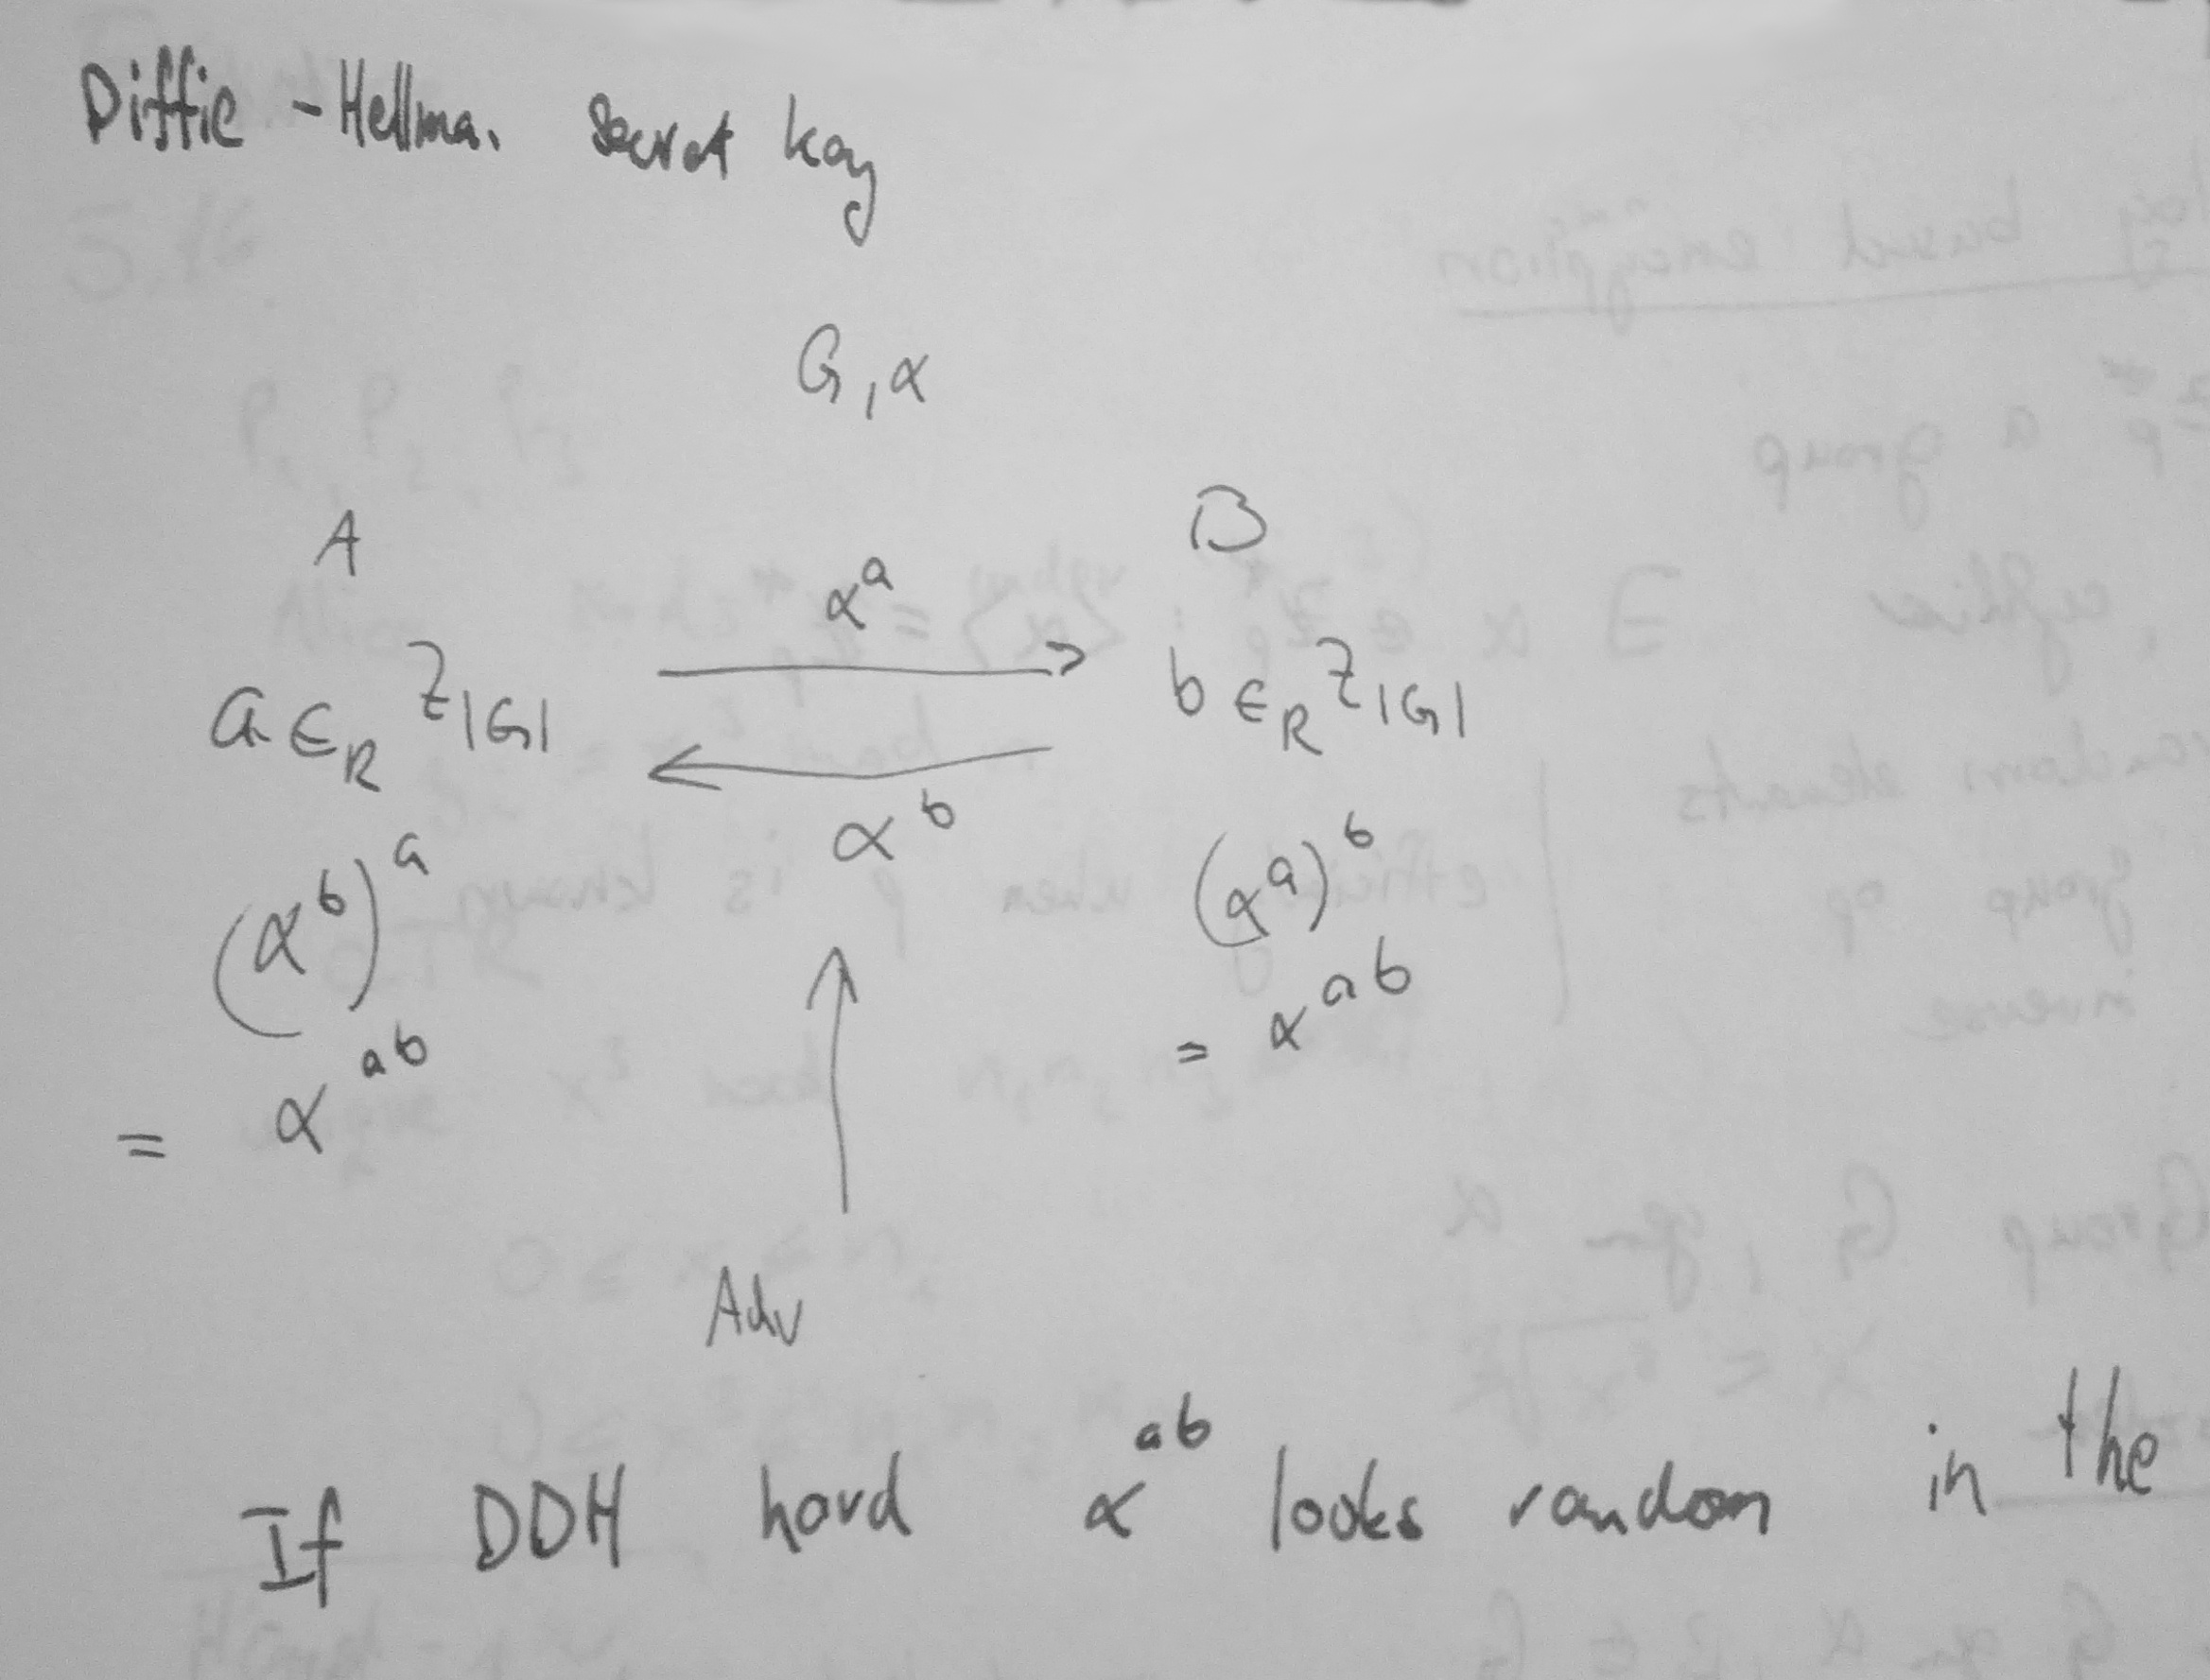
\includegraphics[width=0.5\textwidth]{DH.jpg}
\subsubsection*{El Gamal}
\begin{itemize}
\item 
\textbf{Key generation} On input security parameter \textit{k}, run \textit{GGen} on input \textit{k} to obtain specification of a group \textit{G} and generator $\alpha$. Choose \textit{a} at random from $Z_t$. Then the public key is the specification of \textit{G} and $\beta = \alpha^a$, while the secret key is \textit{a}. The plaintext space is \textit{G} while the ciphertext space is G × G.
\item 
\textbf{Encryption} To encrypt $m \in G$, we choose \textit{r} at random from $Z_t$, and the
ciphertext is $(\alpha^r,\beta^rm)$.
\item 
\textbf{Decryption} To decrypt ciphertext (c,d), compute $c^−ad$.
\end{itemize}
To see that decryption works, simply plug in $(\alpha^r,\beta^rm)$ for $(c,d)$ in the decryption algorithm.

Basic comparisons with previously introduced concepts. Without secret key the El Gamal is 
\subsection*{Definition of CPA security and CPA security of El Gamal}
\textit{Theorem 1 If the DDH problem is hard (w.r.t. GGen), then the El Gamal
cryptosystem is CPA secure.}

The proof of this thing is hand-in no. 9.

\subsection*{Example of groups for use in El Gamal, Zp* does not work but a prime order subgroup does}
\subsubsection*{The $Z^{*}$ is not working}
Lemma 4 $\alpha \in Z^{∗}_p$ is a generator if and only if $\alpha^{(p−1)/q} \neq 1$ for every prime
q that divides p − 1.
Proof:
$$
1 = \alpha^{p−1}\mod p = (\alpha^t)^a \alpha^b \mod p = \alpha^b \mod p.
$$
$$
1 \neq \alpha^{(p−1)/q}\mod p = \alpha^{at/q}\mod p = (\alpha^t)^{a/q}\mod p = 1a/q \mod p = 1
$$
There is possible method how to generate primes that we know the factorization of $p-1$ in the same time. In general we simply take a random prime $q$ a and set $p=2q+1$ and test its primality.

Unfortunately within these groups we can not obtain CPA security.

Lemma 5 Let $\alpha$ be a generator of $Z^{∗}_p$. Then $(\alpha^i)(p−1)/2 \mod p = 1$ if and only if i is even, and is -1 otherwise.

Proof. Clearly $((\alpha^i)^{(p−1)/2})^2 = (\alpha^i)^{p−1} = 1 \mod p$, which implies that
 $(\alpha^i)^{(p−1)/2}$ is 1 or -1 – this follows since $Z_p$ is a field, and so the quadratic
equation $X^2 = 1 \mod p$ can have at most 2 solutions. If $i = 2j$, then
$(\alpha^i)^{(p−1)/2} = (\alpha^{2j})^{(p−1)/2} = (\alpha^j)^{(p−1)}= 1 \mod p$. This gives 
$(p − 1)/2$ elements of $Z_p$ that are solutions to $X^{(p−1)/2} = 1 \mod p$. Again since $Z_p$ is a field, there can be no more, so for all the odd values of $i$, we must have
$(\alpha^i)^{(p−1)/2} \mod p = −1$.

\subsubsection*{Subgroups of $Z^p$}
We will use so called safe primes where $p=2q + 1$. This splits the group into two of order $q$ so if $\alpha_0$ generates the first group $\alpha_0^2$ generates the second half. There is problem with coding, we cannot simply interpret the string as a long number - because that would span the whole group, instead we use a 1-1 mapping.
\begin{itemize}
\item On input $x \in Z_q$, set $y = x + 1$ and compute $y^{(p−1)/2}\mod p$. If this is
1, output $y$, else output $−y \mod p$.
\end{itemize}
\subsubsection*{Other examples}
There are so called ecliptic curves in a form
$$
y^2 = x^3 + ax + b
$$
Where no other algorithm then brute force is know - therefore we can choose much shorter keys (200-300 bits) instead of 1000 we have to use for $Z^{*}_p$.
\end{document}